\documentclass[11pt,a4paper]{article}

\usepackage[margin=2.5cm]{geometry}
\usepackage{amsmath,amssymb,amsthm}
\usepackage{booktabs}
\usepackage{float}
\usepackage{tikz}
\usetikzlibrary{arrows.meta,positioning,calc,fit,backgrounds,decorations.pathreplacing,matrix,shapes.geometric}
\usepackage{pgfplots}
\pgfplotsset{compat=1.18}
\usepackage{microtype}
\usepackage[hidelinks]{hyperref}
\usepackage{xcolor}
\usepackage{enumitem}
\emergencystretch=2em
\setlength{\tabcolsep}{4.5pt}

\definecolor{vcol}{RGB}{31,98,159}
\definecolor{ecol}{RGB}{191,86,24}
\definecolor{gone}{RGB}{150,150,150}
\definecolor{law}{RGB}{32,120,60}
\definecolor{prime}{RGB}{120,60,140}

\newtheorem{definition}{Definition}
\newtheorem{law}{Law}
\newtheorem{proposition}{Proposition}

\newcommand{\tr}{^{\mathsf T}}
\newcommand{\R}{\mathbb R}
\newcommand{\code}[1]{\texttt{#1}}
\newcommand{\ufvm}{\textsc{ufvm}}

\tikzset{
  set/.style={circle, draw=#1, fill=#1!10, thick, minimum size=11mm, font=\small},
  map/.style={-{Stealth[length=2.2mm]}, thick},
  dual/.style={-{Stealth[length=2.2mm]}, thick, dashed, color=law},
  box/.style={draw, rounded corners=2pt, align=left, font=\small\ttfamily, inner sep=5pt},
  pbox/.style={draw=prime, fill=prime!6, rounded corners=2pt, align=left, font=\small, inner sep=5pt, text width=#1},
  lab/.style={font=\small, fill=white, inner sep=1.5pt},
  inst/.style={circle, draw=vcol, fill=vcol!10, thick, minimum size=8mm, font=\small},
  cell/.style={draw, minimum size=9mm, font=\small},
}

\title{\textbf{A Relation-Centred Graph Tower for Finite-Volume Simulation\\ with Exact Derivatives of Any Order}\\[4pt]
\large Architecture, mathematics, verification and an engineering assessment of \ufvm}
\author{Komahan Boopathy\\ \small Technical report, 22 August 2026 --- source at revision \code{db3e31f} with the working tree of this date}
\date{}

\begin{document}
\maketitle

\begin{abstract}
\ufvm{} is a Fortran~2023 library for finite-volume simulation on unstructured meshes in which every object is a composition of eight \emph{prime} types---graph, token, relation, field, operation, transform, map and view---rather than a member of a growing taxonomy of solver classes. The mesh is not stored but \emph{derived}: a file supplies member sets, one cell-to-vertex relation, vertex coordinates and boundary tags, and relation algebra produces faces, incidences and every geometric measurement. A sparse matrix is a weighted relation; a differential operator is a composition of three elementary affine maps between the vertex and edge sets; a time integrator is a traversal of a chain graph; and the adjoint of any compiled operator---in space or in time---is the transpose of the composition, so no reversed kernel exists anywhere in the source. Differentiability is a capability of every operation: a statement declares its exact partial actions once, and tangents, Newton Jacobians, adjoints and forward directional derivatives of arbitrary order are \emph{derived} from them through the chain rule over integer partitions and the implicit function theorem. The same two implicit-function solves serve a time step and a steady spatial residual. We present the mathematical architecture, the design laws that make code disappear, and measurements: the three marching rules reach their nominal orders (1, 1, 2); the discrete adjoint of backward Euler matches its closed form to machine precision and finite differences to $4\times10^{-11}$; second-order directional derivatives in a rate parameter match closed form to $6\times10^{-17}$; the compiled diffusion operator is second order on meshes of $10^2$ to $80^2$ cells; and the 159 property checks of the project's verification suites---removed from the tree in August 2026 and restored from revision \code{ddcf592} by a script shipped with this report---pass against the current source. The assessment also records what is not yet right: operator assembly scales quadratically with cell count, the unpreconditioned Krylov solve scales as $n^{1.7}$, the in-repository test tree was removed, and the distributed runtime is designed but not implemented.
\end{abstract}

\tableofcontents

\section{Introduction}

Scientific simulation codes tend to grow by accretion. A finite-volume solver starts with a mesh class, adds a field class, then a boundary-condition hierarchy, a linear-solver hierarchy, a time-integrator hierarchy, and, much later, sensitivity analysis: tangent and adjoint versions of each of those, produced by hand, by source transformation, or by operator-overloaded tapes. Each addition is a new kind of object with its own invariants, and the coupling between kinds is what makes such codes expensive to extend and hard to verify.

\ufvm{} takes the opposite route. It fixes a small set of irreducible mathematical objects and requires everything else to be a composition, a view, or a concretion of them. The consequence that matters most for engineering is that mathematical laws become \emph{code-elimination mechanisms}: when $(F\circ G)^* = G^*\circ F^*$ is an identity of the representation, the reverse kernel is not written; when a transpose is a view of a relation, the second CSR is not stored; when Newton's Jacobian is the tangent of the statement, no Jacobian is hand-coded; when the dependency graph of a matrix is derivable from its entries, it is not kept. The source as it stands is 63 modules and 21\,450 lines, of which 27\% is prose stating the laws each module keeps.

This report is the first complete description of the system as it exists. It aims to answer four questions a prospective user or maintainer would ask: what the library can do (Section~\ref{sec:features}), on what mathematics it rests (Section~\ref{sec:maths}), what has been verified and measured (Section~\ref{sec:results}), and what is novel about it compared with established frameworks (Sections~\ref{sec:related} and~\ref{sec:discussion}). It closes with an engineering assessment and a prioritized list of future work (Sections~\ref{sec:assessment}--\ref{sec:future}).

\paragraph{Contributions.}
\begin{enumerate}[nosep]
\item A \emph{prime decomposition} of finite-volume simulation into eight types with a stated composition arithmetic, a self-similar kernel graph, and unforgeable identity (Section~\ref{sec:primes}).
\item A \emph{derived mesh}: faces, incidences and all measurements computed by relation algebra from one relation and one coordinate field (Section~\ref{sec:mesh}).
\item \emph{Differentiability as a capability of every operation}: exact partial actions declared once, every derivative object derived---tangent, Jacobian, adjoint, higher-order directional derivatives---with no derivative tensor stored and no automatic-differentiation tool (Section~\ref{sec:diff}).
\item \emph{One affine sparse map} for space and time, carrying composition and transpose once, so the adjoint of a compiled chain is never re-implemented (Section~\ref{sec:affine}).
\item \emph{The implicit function theorem as two routines} that serve a time step and a steady residual identically (Section~\ref{sec:ift}).
\item Verification and measurement of orders of accuracy, derivative exactness and cost, with the scaling defects reported as found (Section~\ref{sec:results}).
\end{enumerate}

\section{Motivation}\label{sec:motivation}

Three recurring problems of simulation software motivated the design.

\paragraph{Taxonomies do not compose.} A class per physical notion---\code{Mesh}, \code{Field}, \code{BoundaryCondition}, \code{Solver}, \code{Integrator}---produces $O(k^2)$ interactions between $k$ kinds, each a special case. The alternative pursued here is to ask which notions are \emph{irreducible}. A mesh is a graph with measurements; a matrix is a graph with weights; a time axis is a graph; a boundary condition is a relation between faces and coefficients. If all of these are one kernel object read through different views, the interactions are theorems rather than cases.

\paragraph{Derivatives are retrofitted.} Sensitivities are usually added after the primal code exists, by a tool that differentiates source text or by a tape that records operations at run time. Both produce a second program whose correctness must be established separately, and neither exploits the structure that the primal already has: that every discrete operator is a composition of a few elementary maps, that a linear map is its own tangent, that an implicit step is one local solve. \ufvm{} makes the partial derivative of a statement part of the statement's contract, and derives everything else.

\paragraph{Time and space are treated by different machinery.} An integrator is written as a loop over steps, a spatial operator as a loop over faces, and their adjoints as two more loops. Both are traversals of a graph in which a local statement reads its neighbours; the adjoint of both is the converse traversal with transposed local blocks. When the representation says so, one implementation serves both.

The governing principle, stated in the repository's constitution and enforced in its source, is: \emph{prove structure once; delete the corresponding cases from the implementation.}

\section{Related work and positioning}\label{sec:related}

\paragraph{Finite-volume frameworks.} OpenFOAM~\cite{weller1998} and SU2~\cite{economon2016} are the reference open-source unstructured finite-volume codes. Both store the mesh explicitly (owner/neighbour or cell-face adjacency arrays) and express discretizations through operator objects that assemble matrices. SU2 obtains discrete adjoints by operator-overloading algorithmic differentiation (CoDiPack~\cite{sagebaum2019}) of the whole primal iteration; OpenFOAM's adjoint solvers are hand-derived continuous or discrete adjoints per physics. In \ufvm{} the mesh is derived from one relation, matrices are weighted relations, and the adjoint of a compiled operator is its transpose.

\paragraph{Finite-element frameworks with symbolic forms.} FEniCS~\cite{logg2012}, Firedrake~\cite{rathgeber2016} and MFEM~\cite{anderson2021} express variational forms symbolically (UFL) or through operator classes and generate kernels. dolfin-adjoint/pyadjoint~\cite{farrell2013,mitusch2019} derive discrete adjoints by recording the sequence of solves on a tape and reversing it; higher-order derivatives are obtained by taping the tangent. \ufvm{} shares the idea that the derivative should follow from the structure of the forward computation, but realizes it without a tape: each operation declares its exact partial actions, and the chain rule to any order is assembled from integer partitions at the call.

\paragraph{Time integration with sensitivities.} SUNDIALS CVODES/IDAS~\cite{hindmarsh2005} and PETSc TS with TSAdjoint~\cite{zhang2022} provide forward and adjoint sensitivities of multistep and Runge--Kutta integrators, with hand-derived adjoint formulas per method family. In \ufvm{} the $\theta$-scheme and BDF family are one operation whose partials are derived from the action's, and the adjoint march is the converse traversal with the transposed compiled block; no integrator has an adjoint of its own.

\paragraph{Algorithmic differentiation.} Source transformation (Tapenade~\cite{hascoet2013}), operator overloading (ADOL-C~\cite{griewank1996}, CoDiPack), compiler-level differentiation (Enzyme~\cite{moses2020}) and array-language transformation (JAX~\cite{jax2018}) differentiate programs. \ufvm{} differentiates \emph{statements}: the unit is a mathematical operation with a declared argument space, and the derivative machinery is structural (composition, transpose, partitions) rather than program-level. The approach is closer in spirit to Griewank and Walther's treatment of higher-order derivatives through Taylor arithmetic~\cite{griewank2008} and to Faà di Bruno's formula, which the chain-rule module implements directly.

\paragraph{Discrete exterior calculus.} The three elementary steps---average, difference, incidence---are the 0- and 1-cochain operators of discrete exterior calculus~\cite{desbrun2005,hirani2003,bell2012}. \ufvm{} does not adopt the full DEC vocabulary; it keeps the operators as affine maps between two finite sets so that the boundary value enters the constant and the adjoint is the transpose of the composition.

\paragraph{Relational and graph-based formulations.} Treating the mesh as relations between sets and deriving incidence by relational algebra is familiar from the database view of meshes and from the topological data structures literature~\cite{garimella2002}. \ufvm{} takes it further: relations are first-class with identity, the partition of a graph is one relation read in two directions, and a weighted relation is the matrix.

Table~\ref{tab:compare} summarizes the positioning on the axes that distinguish the design. The table records mechanisms, not quality; each of the systems named is far more complete in physics and scale than \ufvm{} today.

\begin{table}[htbp]
\centering\footnotesize
\begin{tabular}{@{}p{2.3cm}p{3.0cm}p{3.0cm}p{3.0cm}p{3.4cm}@{}}
\toprule
Axis & OpenFOAM, SU2 & FEniCS, Firedrake & SUNDIALS, PETSc TS & \ufvm \\
\midrule
Mesh & stored adjacency arrays & stored topology & n/a & derived from one relation and one field \\
Matrix & sparse storage class & sparse storage class & PETSc Mat & weighted relation; pattern derived \\
Derivative mechanism & hand adjoints; AD by overloading (SU2) & symbolic forms; tape (pyadjoint) & hand-derived per method & declared partial actions; structural composition \\
Adjoint of an operator chain & differentiated program & reversed tape & method-specific formulas & transpose of the composed map \\
Higher-order derivatives & tape of tape & tape of tape & second order (TSAdjoint) & any order, Faà di Bruno over partitions \\
Time vs.\ space & separate machinery & separate machinery & time only & one traversal, one implicit-function solve \\
Language & C++ & Python/C++ & C & Fortran 2023 \\
\bottomrule
\end{tabular}
\caption{Positioning by mechanism. The comparison is about how each system represents and differentiates, not about scope or maturity.}
\label{tab:compare}
\end{table}

\section{The mathematical architecture}\label{sec:maths}

\subsection{Eight primes and the composition arithmetic}\label{sec:primes}

\begin{definition}[prime]
A type is \emph{prime} when it cannot be expressed as a composition of the others. Everything that is not prime must say which primes it composes.
\end{definition}

The eight primes and the arithmetic that generates the rest are shown in Figure~\ref{fig:tower}. The statement that every higher type is a composition is enforced by two mechanical checks on the source: the build order of the 63 modules is a linear extension of their dependency graph (a file may import only modules built before it), and the naming law assigns every module to a prime namespace.

\begin{figure}[H]
\centering
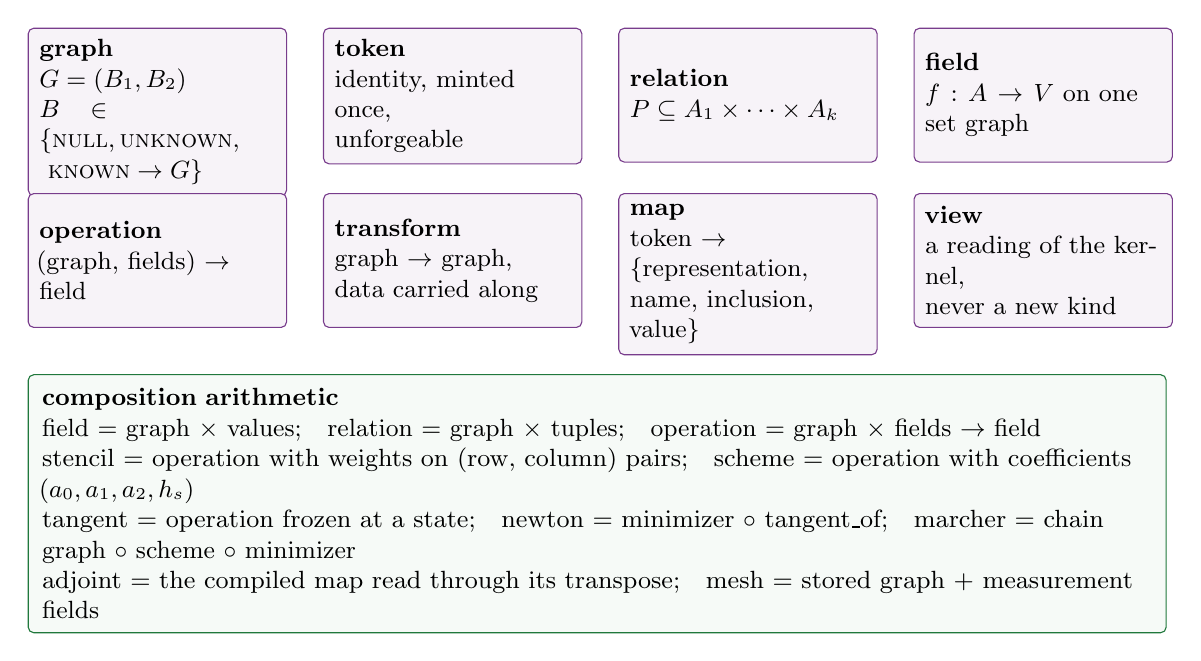
\begin{tikzpicture}
  \tikzset{pb/.style={draw=prime, fill=prime!6, rounded corners=2pt, align=left, font=\small, inner sep=4pt, text width=3.0cm, minimum height=17mm, anchor=north west}}
  \node[pb] (graph) at (0,0) {\textbf{graph}\\ $G=(B_1,B_2)$\\ $B\in\{\textsc{null},\textsc{unknown},$\\ $\ \textsc{known}\to G\}$};
  \node[pb] (token) at (3.75,0) {\textbf{token}\\ identity, minted once,\\ unforgeable};
  \node[pb] (relation) at (7.5,0) {\textbf{relation}\\ $P\subseteq A_1\times\cdots\times A_k$};
  \node[pb] (field) at (11.25,0) {\textbf{field}\\ $f:A\to V$ on one set graph};
  \node[pb] (operation) at (0,-2.1) {\textbf{operation}\\ (graph, fields) $\to$ field};
  \node[pb] (transform) at (3.75,-2.1) {\textbf{transform}\\ graph $\to$ graph,\\ data carried along};
  \node[pb] (mapp) at (7.5,-2.1) {\textbf{map}\\ token $\to$ \{representation,\\ name, inclusion, value\}};
  \node[pb] (view) at (11.25,-2.1) {\textbf{view}\\ a reading of the kernel,\\ never a new kind};
  \node[draw=law, fill=law!4, rounded corners=2pt, align=left, font=\small, inner sep=5pt, text width=14.1cm, anchor=north west] at (0,-4.4) {
  \textbf{composition arithmetic}\\
  field $=$ graph $\times$ values;\quad relation $=$ graph $\times$ tuples;\quad operation $=$ graph $\times$ fields $\to$ field\\
  stencil $=$ operation with weights on (row, column) pairs;\quad scheme $=$ operation with coefficients $(a_0,a_1,a_2,h_s)$\\
  tangent $=$ operation frozen at a state;\quad newton $=$ minimizer $\circ$ tangent\_of;\quad marcher $=$ chain graph $\circ$ scheme $\circ$ minimizer\\
  adjoint $=$ the compiled map read through its transpose;\quad mesh $=$ stored graph $+$ measurement fields};
\end{tikzpicture}
\caption{The eight primes and the arithmetic by which every other type is formed. The kernel graph is self-similar: sets, tuples, relations, domains and chains are this one object read differently, and there is exactly one type named \code{graph}.}
\label{fig:tower}
\end{figure}

\subsection{The kernel graph and identity}\label{sec:kernel}

The kernel is deliberately minimal (Figure~\ref{fig:kernel}). A graph is a pair of branches; a branch is \textsc{null}, \textsc{unknown}, or a reference to another graph. The three states are values, not subtypes; the status and the reference are private, so the invariant
\[
\text{status} = \textsc{known} \iff \text{the reference is associated}
\]
can only be established by the three constructors and cannot be broken by a caller. \textsc{unknown} is distinct from \textsc{null}: a halo before exchange is not absent, and an empty set is not unknown.

Identity is a service beneath the tower. A token is an (image, serial) pair with private components, so the only ways a token exists are minting and copying: a copy \emph{is} the identity, and two coarray images can never mint the same stamp. Every map in the system is keyed on identity tokens copied at attachment, never on storage position, so containers may grow, reorder or compact without redirecting an attachment. This separates two questions that simulation codes habitually conflate:
\[
\text{identity (which set?)} \quad\neq\quad \text{extension (which members?)}.
\]
Two independently declared sets over $\{1,\dots,8\}$ are equivalent and are not the same set; a transposed relation signs its own token and is never \code{same\_as} its base even though it has the same tuples.

\begin{figure}[H]
\centering
\resizebox{0.96\textwidth}{!}{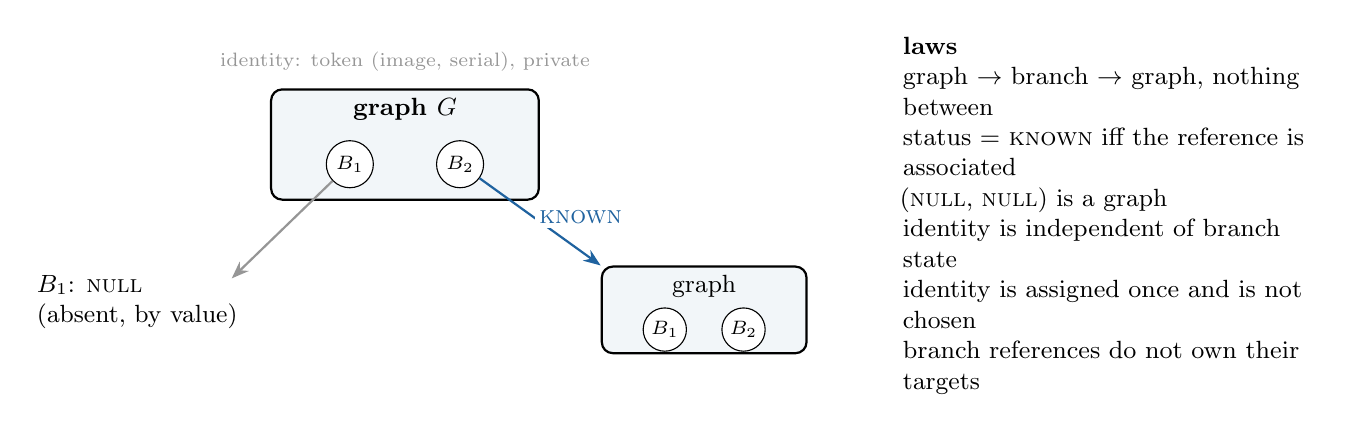
\begin{tikzpicture}
  \node[draw, rounded corners, thick, fill=vcol!6, minimum width=34mm, minimum height=14mm] (G) at (0,0) {};
  \node[font=\small\bfseries] at (0,0.45) {graph $G$};
  \node[draw, circle, fill=white, inner sep=2pt, font=\scriptsize] (b1) at (-0.7,-0.25) {$B_1$};
  \node[draw, circle, fill=white, inner sep=2pt, font=\scriptsize] (b2) at (0.7,-0.25) {$B_2$};
  \node[font=\scriptsize, gone] at (0,1.05) {identity: token (image, serial), private};
  \node[draw, rounded corners, thick, fill=vcol!6, minimum width=26mm, minimum height=11mm] (G2) at (3.8,-2.1) {};
  \node[font=\small] at (3.8,-1.8) {graph};
  \node[draw, circle, fill=white, inner sep=1.5pt, font=\scriptsize] at (3.3,-2.35) {$B_1$};
  \node[draw, circle, fill=white, inner sep=1.5pt, font=\scriptsize] at (4.3,-2.35) {$B_2$};
  \draw[map, vcol] (b2) -- node[lab, right, pos=.45]{\textsc{known}} (G2.north west);
  \node[font=\small, align=left] at (-3.4,-2.0) {$B_1$: \textsc{null}\\ (absent, by value)};
  \draw[map, gone] (b1) -- (-2.2,-1.7);
  \node[align=left, font=\small, text width=5.4cm, anchor=west] at (6.2,-0.9) {
  \textbf{laws}\\
  graph $\to$ branch $\to$ graph, nothing between\\
  status $=$ \textsc{known} iff the reference is associated\\
  (\textsc{null}, \textsc{null}) is a graph\\
  identity is independent of branch state\\
  identity is assigned once and is not chosen\\
  branch references do not own their targets};
\end{tikzpicture}}
\caption{The kernel graph. Sets, sequences, relational graphs and epistemic (data, operator) pairs are \emph{views} of this object; the view that reads a graph as a set stores the extension in a representation outside the graph, so a set of $N$ members is $O(1)$ semantic objects, not $O(N)$.}
\label{fig:kernel}
\end{figure}

\subsection{Sets, maps and views}

A set is a graph read through a \emph{representation} held in a map: \code{num\_members}, \code{member(k)} and \code{local\_index(v)} bound by the enumeration laws
\[
\code{member}(\code{local\_index}(v)) = v,\qquad \code{local\_index}(\code{member}(k)) = k,
\]
from which membership and the member list are theorems answered once for every concretion. A counted representation answers \code{local\_index} in $O(1)$; a listed one scans. Three further maps record what a set is called, which ambient set a subset is declared into (the inclusion is the identity on values, so only the \emph{association} is stored), and which value field is attached to a graph with what trust status. All are keyed on identity and stored outside the graph.

\subsection{Relations}\label{sec:relations}

A relation is a named finite-arity subset $P\subseteq A_1\times\cdots\times A_k$ with identity, an ordered signature of set graphs, and a membership law; it is first-class and needs no graph to exist. Arity two earns its own contract because it has its own questions: \code{source}, \code{target}, \code{image(a)}, \code{preimage(b)}. The CSR concretion stores both directions once at construction, so each fibre is one row slice and construction is linear in members plus tuples; every query speaks member values, never storage rows, and the cost is stated parametrically, $T_{\text{image}}(a) = T_{\text{local\_index}}(a) + O(\deg a)$.

\begin{law}[transpose is a view]
\code{transpose\_of}$(P)$ is an $O(1)$ view that borrows its base: image and preimage swapped, the signature read in reverse. The involution $(P\tr)\tr = P$ is a statement about extension, not identity.
\end{law}

One grouping kernel---a counting sort that fibres a tuple list over one slot---builds the CSR, the incidence lists, the padded transpose and the combination of duplicate matrix entries; no other count/prefix/scatter exists in the source. The relation algebra module holds exactly the three primitives its first caller earned (restriction, projection, binary composition); graph algorithms (sources, sinks, reachability, topological order with loud refusal on a cycle) act on a relation from outside, as free procedures, never as methods.

\subsection{The partition relation}\label{sec:partition}

A cut and an assembly are not two records but one relation read in two directions, $r\subseteq S_{\text{part}}\times S_{\text{whole}}$, one per carrier (vertices, edges). The partitioner writes it; the assembler is handed it and never invents one. The law the pair satisfies,
\[
\text{assemble}(\text{partition}(G)) = G,\qquad \text{assemble}(\text{partition}(G,D)) = (G,D),
\]
is exact in both directions; coarsen/refine satisfy the one-sided law $\text{coarsen}(\text{refine}(G)) = G$. A part owns the cells it answers for and borrows the neighbours it must see; only owned values are collected, because collecting a borrowed copy would count a conserved quantity twice---exactly at a partition boundary, where the error is hardest to locate (Figure~\ref{fig:partition}).

\begin{figure}[H]
\centering
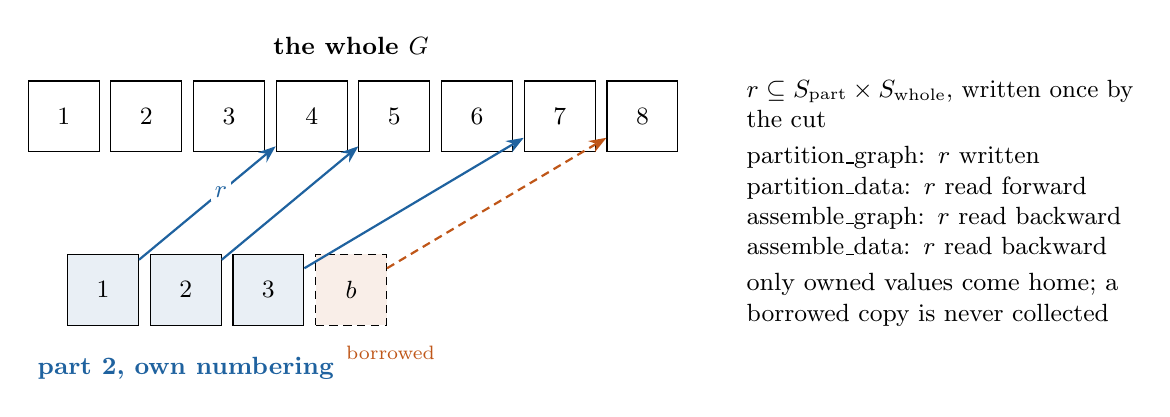
\begin{tikzpicture}[x=1cm,y=1cm]
  \foreach \i in {1,...,8} { \node[cell] (w\i) at (\i*1.05,0) {$\i$}; }
  \node[font=\small\bfseries] at (4.7,0.9) {the whole $G$};
  \foreach \i in {1,2,3} { \node[cell, fill=vcol!10] (p\i) at (\i*1.05+0.5,-2.2) {$\i$}; }
  \node[cell, fill=ecol!10, densely dashed] (pb) at (4*1.05+0.5,-2.2) {$b$};
  \node[font=\small\bfseries, vcol] at (2.6,-3.2) {part 2, own numbering};
  \node[font=\scriptsize, ecol] at (5.2,-3.0) {borrowed};
  \draw[map, vcol] (p1) -- node[lab,pos=.6]{$r$} (w4);
  \draw[map, vcol] (p2) -- (w5);
  \draw[map, vcol] (p3) -- (w7);
  \draw[map, ecol, densely dashed] (pb) -- (w8);
  \node[align=left, font=\small, text width=4.9cm, anchor=west] at (9.6,-1.1) {
  $r\subseteq S_{\text{part}}\times S_{\text{whole}}$, written once by the cut\\[2pt]
  partition\_graph: $r$ written\\ partition\_data: $r$ read forward\\ assemble\_graph: $r$ read backward\\ assemble\_data: $r$ read backward\\[2pt]
  only owned values come home; a borrowed copy is never collected};
\end{tikzpicture}
\caption{The partition relation. One value drives all four motions; the round-trip law is exact. The suite verifies, for 1--3 parts, that every assembled edge is an edge of $G$ and every edge of $G$ is assembled by some part, that $\sum_k A_k(P_k(D)) = D$ on vertex and edge data, that every cell is owned exactly once, and that a part handed the wrong relation is \emph{refused by identity}, the two relations being indistinguishable by size.}
\label{fig:partition}
\end{figure}

\subsection{Fields, reductions and the parallel law}

A field is a function over one finite domain named by a set graph; it keeps the domain's identity and a frozen count, nothing else, so $N$ fields on one domain do not hold $N$ copies of its extension. A functional is the field at domain size one; it carries real, complex (so a complex-step derivative survives a reduction) and logical values.

A reduction turns a field into a number in four steps---accumulate, combine, finalize, with a measure---because the graph may be in pieces. The average of part-averages is wrong; the sum and the count must travel together and divide once at the end. Minimum and maximum are safe to finish early, average and norm are not, so every rule uses the four steps. With a measure a bare sum becomes an integral, and the measure position is also the inner product's second field, which is how the Krylov solvers obtain $\langle q, v\rangle$ from the reduction. This is the parallel law, designed in before any parallel code exists.

\subsection{Operations and differentiability}\label{sec:diff}

An operation is the verb within a graph: $(\text{graph}, \text{fields}) \to \text{field}$, with three symbols---\code{name}, \code{domain} (which set the result lives on and how many entries) and \code{apply}. A concrete operation is handed the fields it reads at construction; \code{apply} fetches nothing by name.

The operation also owns an \emph{argument space}. $F(x_1,\dots,x_m)$ reads inputs by position; \code{declare\_arguments}$(m)$ fixes the readable positions; an argument is an opaque ordinal in one operation's space, and two arguments match only when they name the same position of the same space---an argument of another operation can never stand for one of this operation's. A \emph{variation} is one factor $(a_j, v_j)$, an argument and a direction. Every operation reports
\[
\code{max\_degree},\qquad \code{partial\_action}(x, [(a_1,v_1),\dots,(a_k,v_k)]) = D_{a_1}\cdots D_{a_k}F(x)[v_1,\dots,v_k],
\]
the mixed partial contracted against its directions, on the operation's own domain. The default \code{max\_degree} is 0 and the default partial stops the program: an operation that declares no calculus has none. No derivative tensor is ever stored.

Everything that is a derivative is then derived (Figure~\ref{fig:derived}):
\begin{itemize}[nosep]
\item the \emph{linearization} $D_aS(x)[v]$ at a frozen input tuple, behind the operation interface so a minimizer sees a linear operation; exact through \code{partial\_action} when \code{max\_degree}$\ge1$, by differences of two residuals otherwise---one dispatch, the primal written once;
\item \emph{Newton} as a minimizer whose Jacobian action is \code{tangent\_of}(action), owning no derivative mathematics;
\item the \emph{chain rule to any order}: for $S(x_1(s),\dots,x_m(s))$, $d^n/ds^n$ is assembled from the exact partial actions over integer partitions $d=[d_1,\dots,d_k]$ of $n$ with the multinomial count $c(d) = n!/(\prod_i d_i!\,\prod_j \mathrm{mult}_j!)$, partitions generated rather than tabulated; an unoccupied path derivative reads as zero;
\item the \emph{scheme's} partials from the action's (Section~\ref{sec:scheme}), the \emph{stencil's} tangent as itself (a linear map), and the \emph{implicit function theorem} (Section~\ref{sec:ift}).
\end{itemize}

\begin{figure}[H]
\centering
\resizebox{\textwidth}{!}{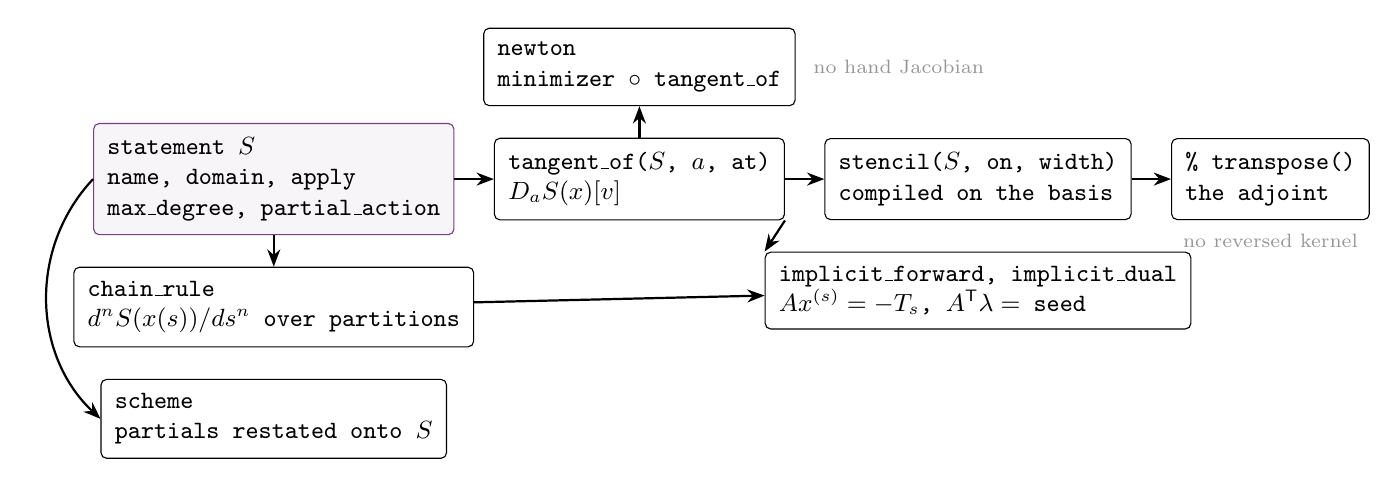
\begin{tikzpicture}[node distance=4mm and 5mm, every node/.append style={font=\scriptsize\ttfamily}]
  \node[box, draw=prime, fill=prime!5] (S) {statement $S$\\ name, domain, apply\\ max\_degree, partial\_action};
  \node[box, right=of S] (tan) {tangent\_of($S$, $a$, at)\\ $D_aS(x)[v]$};
  \node[box, above=of tan] (newton) {newton\\ minimizer $\circ$ tangent\_of};
  \node[box, right=of tan] (st) {stencil($S$, on, width)\\ compiled on the basis};
  \node[box, right=of st] (adj) {\% transpose()\\ the adjoint};
  \node[box, below=of st] (ift) {implicit\_forward, implicit\_dual\\ $A x^{(s)} = -T_s$,\ $A\tr\lambda=$ seed};
  \node[box, below=of S] (cr) {chain\_rule\\ $d^n S(x(s))/ds^n$ over partitions};
  \node[box, below=of cr] (sch) {scheme\\ partials restated onto $S$};
  \draw[map] (S) -- (tan); \draw[map] (tan) -- (newton); \draw[map] (tan) -- (st); \draw[map] (st) -- (adj); \draw[map] (tan.south east) -- (ift.north west);
  \draw[map] (S) -- (cr); \draw[map] (S.west) to[bend right=45] (sch.west); \draw[map] (cr) -- (ift);
  \node[below=0.5mm of adj, font=\scriptsize, gone] {no reversed kernel};
  \node[right=1mm of newton, font=\scriptsize, gone] {no hand Jacobian};
\end{tikzpicture}}
\caption{One primal, every derivative derived. The statement declares its exact partials once; tangent, Newton, compiled matrix, adjoint, total derivatives of any order and the implicit-function solves are built from them.}
\label{fig:derived}
\end{figure}

\subsection{The affine sparse map}\label{sec:affine}

\begin{definition}
An affine sparse map between finite sets $C$ (columns) and $R$ (rows) is $\phi=(A,k):\R^C\to\R^R$, $\phi(q)=Aq+k$, with $A$ a weighted relation $A\subseteq R\times C$ and $k\in\R^R$ the constant the boundary values leave behind.
\end{definition}

The \code{stencil} is this object: triples $(r,c,w)$, constants, two extents, and the two domains when its maker knows them. Two laws are written once:
\begin{law}[composition]\label{law:comp}
$(A_2,k_2)\circ(A_1,k_1) = (A_2A_1,\ A_2k_1+k_2)$, by sparse triple product with duplicate pairs combined.
\end{law}
\begin{law}[transpose]\label{law:tr}
$(A,k)\tr = (A\tr,0)$: the adjoint acts on the linear part.
\end{law}
\begin{proposition}\label{prop:norev}
$(\phi_n\circ\cdots\circ\phi_1)\tr = \phi_1\tr\circ\cdots\circ\phi_n\tr$ on the linear parts; hence no reversed kernel need exist---the transpose is taken once, after the chain is composed.
\end{proposition}

The dependency graph---one edge per entry, column to row---is what a colouring and a Galerkin coarsening read; it is derived on request and not stored, the same law the directed graph applies to its own relations after a benchmark caught eager materialization costing every construction $2.2\times$. A stencil is also compiled from any operation by evaluation on the standard basis (zero state $\to$ constant; $e_j$ minus constant $\to$ column $j$), with a rectangular column side when the operation's argument lives on another domain.

\paragraph{The parity chain.} On a directed graph $(V,E)$ three elementary steps move values between the two sets (Figure~\ref{fig:parity}): the average $S:\R^V\to\R^E$, the difference $G:\R^V\to\R^E$, $z_e = c\,(q_j-q_i)/h_e$, and the incidence $D:\R^E\to\R^V$, $y_v = (\text{out}-\text{in})/m_v$. An edge with no head is a boundary face; its missing end reads the boundary value into the constant. The operator of order $n$ is
\[
\text{vertex}(2k) = (DG)^k,\qquad \text{vertex}(2k{+}1) = (DG)^kDS,\qquad \text{edge}(n) = G\,\text{vertex}(n{-}1),
\]
with the coefficient carried by the innermost step, so that a per-edge coefficient makes order 2 the operator $\nabla\!\cdot(k\nabla q)$. Each step consults an edge's two ends, so order $n$ reaches exactly $n$ rings of neighbours. Exactness is claimed on the uniform chain, where the discrete formulas coincide with calculus (the second derivative is exact on a parabola, order four on $x^4$), and verified there.

\begin{figure}[H]
\centering
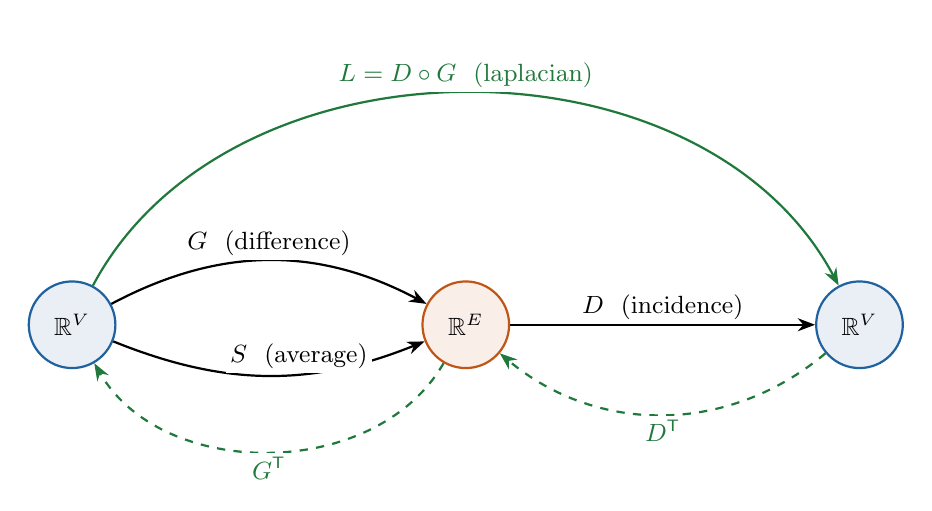
\begin{tikzpicture}
  \node[set=vcol] (V) at (0,0) {$\R^{V}$};
  \node[set=ecol] (E) at (5,0) {$\R^{E}$};
  \node[set=vcol] (V2) at (10,0) {$\R^{V}$};
  \draw[map] (V) to[bend left=28] node[lab,above]{$G$ \ (difference)} (E);
  \draw[map] (V) to[bend right=22] node[lab,above,pos=.6]{$S$ \ (average)} (E);
  \draw[map] (E) -- node[lab,above]{$D$ \ (incidence)} (V2);
  \draw[dual] (V2) to[bend left=40] node[lab,below]{$D\tr$} (E);
  \draw[dual] (E) to[bend left=60] node[lab,below]{$G\tr$} (V);
  \draw[map, law, thick] (V) to[bend left=62] node[lab,above]{$L = D\circ G$ \ (laplacian)} (V2);
\end{tikzpicture}
\caption{The parity chain. Solid arrows are the three step stencils, the green arc their composition; dashed arrows are the transposes, never written as kernels. $L\tr = (D\circ G)\tr = G\tr\circ D\tr$ is checked numerically in the demonstration \code{demo/law.f90}.}
\label{fig:parity}
\end{figure}

\subsection{The scheme and the chain graph}\label{sec:scheme}

Time is a chain graph: instants are vertices, steps are edges, a step size is a number per edge. The $\theta$-scheme residual over an action $S$ (which returns minus the velocity) is one operation,
\[
R(q_n,\xi,q_{n-1},q_{n-2}) = a_0q_n + a_1q_{n-1} + a_2q_{n-2} + h\big[\theta S(q_n,\xi) + (1-\theta)S(q_{n-1},\xi)\big],
\]
with $\theta=1$ backward Euler and BDF2, $\theta=0$ forward Euler, $\theta=\tfrac12$ Crank--Nicolson, and variable-step BDF2 coefficients $a_0 = (2h_0+h_1)/(h_0+h_1)$, $a_1=-(h_0+h_1)/h_1$, $a_2 = h_0^2/(h_1(h_0+h_1))$. The scheme's argument space is the action's followed by its history; every partial of $R$ is derived from the action's partial actions by the formula above, each variation restated on the action's argument first, so the tangent of the step equation is exact when $S$'s is. No scheme-specific derivative code exists, and \code{bdf\_variable} inherits it.

\subsection{The implicit function theorem, once}\label{sec:ift}

Let $R(x_1,\dots,x_m)=0$ be held at its input tuple and solved in argument $a$, with $A=D_aR$ compiled at the tuple. Then
\begin{align}
\text{forward:}&\qquad A\,x_a^{(s)} = -T_s,\qquad T_s = \text{the chain-rule total of order $s$ with } x_a^{(s)}=0, \label{eq:fwd}\\
\text{dual:}&\qquad A\tr\lambda = \text{seed},\qquad g_b = (D_bR)\tr\lambda \ \text{ for every other argument } b. \label{eq:dual}
\end{align}
\code{implicit\_forward} and \code{implicit\_dual} are these two solves; the block is compiled once to a stencil, the solver is the caller's minimizer (dense direct for a $3\times3$ time step, CG or GMRES for a large spatial residual), and with a diagonal block nothing is compiled (an explicit scheme). The dual of any block, square or rectangular, is the transpose of the compiled tangent on that argument's own domain.

\subsection{The marcher as a traversal}\label{sec:marcher}

The marcher owns the traversal and the seeds (Figure~\ref{fig:march}). Forward: at each edge, one local solve of the scheme with the history held (by the residual at zero over $-a_0$ when $\theta=0$, by the held minimizer otherwise). Directional: at each edge, one call of~\eqref{eq:fwd} with the history paths holding every solved derivative of the earlier instants. Adjoint: the converse traversal; every instant carries a seed $\sigma_v$, and at edge $e$ with $v=e+1$ one call of~\eqref{eq:dual} answers $\lambda_e$ and the duals $g_k$ of the history blocks, after which $\sigma_{v-k}\leftarrow\sigma_{v-k}-g_k$ for $k$ up to the reach. Adaptive marching separates mechanism from decision: the marcher computes a trial and an error estimate; a policy proposes, judges and retries from scalars alone.

\begin{figure}[H]
\centering
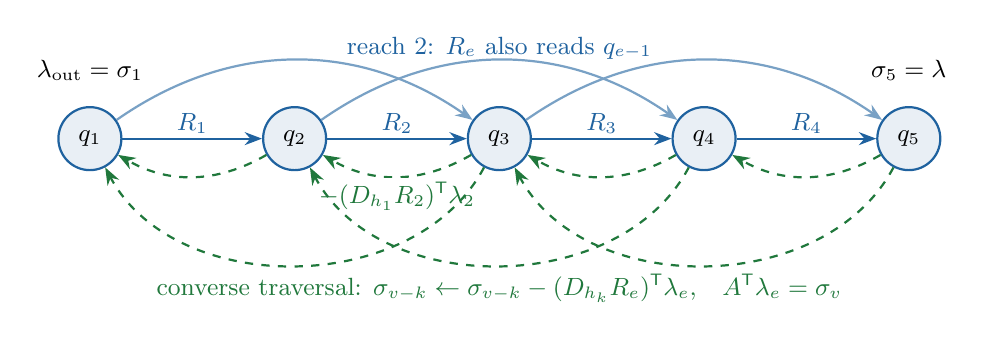
\begin{tikzpicture}[x=2.6cm]
  \foreach \i in {1,...,5} { \node[inst] (q\i) at (\i,0) {$q_\i$}; }
  \foreach \i/\j in {1/2,2/3,3/4,4/5} { \draw[map, vcol] (q\i) -- node[lab,above]{$R_\i$} (q\j); }
  \foreach \i/\j in {1/3,2/4,3/5} { \draw[map, vcol!60, bend left=35] (q\i) to (q\j); }
  \node[font=\small, vcol] at (3,1.15) {reach 2: $R_e$ also reads $q_{e-1}$};
  \foreach \i/\j in {5/4,4/3,2/1} { \draw[dual, bend left=30] (q\i) to (q\j); }
  \draw[dual, bend left=30] (q3) to node[lab,below]{$-(D_{h_1}R_2)\tr\lambda_2$} (q2);
  \foreach \i/\j in {5/3,4/2,3/1} { \draw[dual, bend left=62] (q\i) to (q\j); }
  \node[font=\small, law] at (3,-1.9) {converse traversal: $\sigma_{v-k} \leftarrow \sigma_{v-k} - (D_{h_k}R_e)\tr\lambda_e$,\quad $A\tr\lambda_e = \sigma_v$};
  \node[above=2mm of q5, font=\small] {$\sigma_5=\lambda$};
  \node[above=2mm of q1, font=\small] {$\lambda_{\text{out}}=\sigma_1$};
\end{tikzpicture}
\caption{The marcher. Forward (blue): one implicit-function solve per edge. Converse (green, dashed): the same block transposed; each history dual is subtracted from the seed of the instant it reads. The accumulation is over the dependencies that read an instant, the form that survives on a graph that is not a chain.}
\label{fig:march}
\end{figure}

\subsection{Minimizers and multigrid}

Every solver is a \emph{minimizer}: attach a statement, drive its residual on the residual domain to zero by varying values on the unknown domain. The solver vocabulary---\code{matvec}, \code{inner\_product}, \code{norm}, \code{sweep\_order}, \code{diagonal}, \code{constant}---is defined once as delegations to the engine (the operation, the reductions, the colouring walk), so a concrete solver states only its iteration: Jacobi, Gauss--Seidel swept by colour (SOR is $\omega\ne1$, a parameter, not a solver), conjugate gradients, restarted GMRES, dense direct elimination, Newton, and two-grid multigrid. The diagonal is probed by colour: the operator applied to one colour's indicator answers the diagonal at every member of that colour, because no two neighbours share a colour. Multigrid's coarse operator is the fine stencil read through the aggregates---$RAP$ with summing restriction and injected prolongation---obtained by relabelling the triples and combining duplicates; the suite holds the commutation square, \emph{coarsen-then-solve returns $e$}.

\subsection{The mesh, derived}\label{sec:mesh}

A mesh file supplies member sets (vertices, cells, tagged boundary faces), one relation $C2V\subseteq \text{cells}\times\text{vertices}$, one field (coordinates), and labels. Everything a finite-volume solver reads is derived (Figure~\ref{fig:mesh}): interior faces as shared-vertex intersections of cell pairs; $V2C = C2V\tr$ by the padded transpose; $F2C = \{(f,c): F2V(f)\subseteq C2V(c)\}$ with at most two cells per face, one cell meaning a boundary face; and the measurements as fields---centres, volumes, areas, normals, centre-to-centre deltas, interpolation weights. The mesh is the tower's one inheritance crossing: it \emph{is} a directed graph whose vertices are cells and whose edges are two-cell faces, boundary faces being edges without heads. No string names a measurement; an operator receives the numbers at construction and never reads the mesh. The loader reads gmsh MSH~4.1.

\begin{figure}[H]
\centering
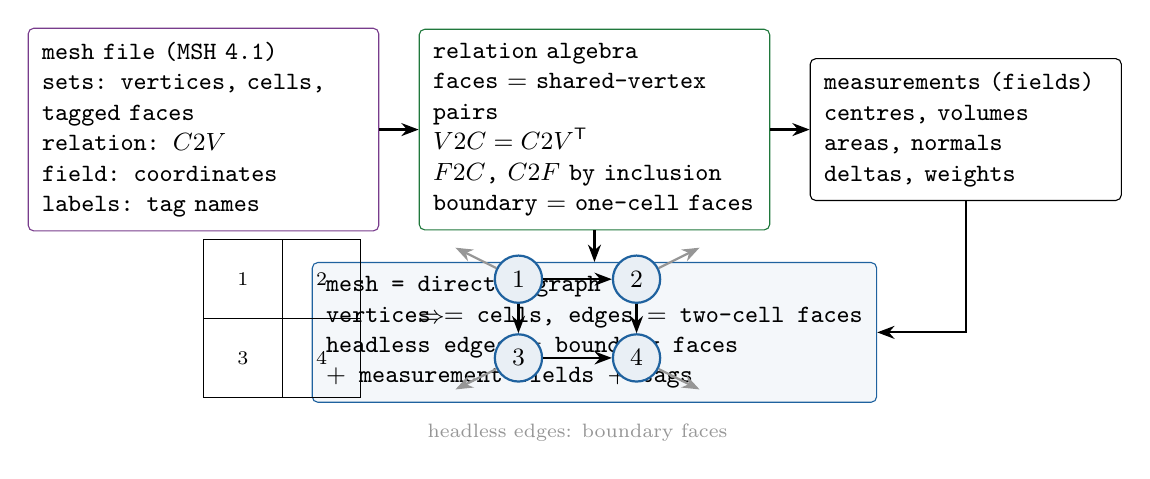
\begin{tikzpicture}[node distance=4mm and 5mm]
  \node[box, draw=prime, text width=4.1cm] (file) {mesh file (MSH 4.1)\\ sets: vertices, cells, tagged faces\\ relation: $C2V$\\ field: coordinates\\ labels: tag names};
  \node[box, right=of file, draw=law, text width=4.1cm] (alg) {relation algebra\\ faces $=$ shared-vertex pairs\\ $V2C = C2V\tr$\\ $F2C$, $C2F$ by inclusion\\ boundary $=$ one-cell faces};
  \node[box, right=of alg, text width=3.6cm] (geo) {measurements (fields)\\ centres, volumes\\ areas, normals\\ deltas, weights};
  \node[box, below=of alg, draw=vcol, fill=vcol!5] (mesh) {mesh = directed graph\\ vertices $=$ cells, edges $=$ two-cell faces\\ headless edges $=$ boundary faces\\ $+$ measurement fields $+$ tags};
  \draw[map] (file) -- (alg); \draw[map] (alg) -- (geo); \draw[map] (alg) -- (mesh); \draw[map] (geo) |- (mesh);
  % picture of the mesh
  \begin{scope}[shift={(0,-3.4)}]
    \draw (0,0) grid[step=1] (2,2);
    \node[font=\scriptsize] at (0.5,1.5) {1}; \node[font=\scriptsize] at (1.5,1.5) {2};
    \node[font=\scriptsize] at (0.5,0.5) {3}; \node[font=\scriptsize] at (1.5,0.5) {4};
    \node[inst, minimum size=6mm] (c1) at (4,1.5) {1}; \node[inst, minimum size=6mm] (c2) at (5.5,1.5) {2};
    \node[inst, minimum size=6mm] (c3) at (4,0.5) {3}; \node[inst, minimum size=6mm] (c4) at (5.5,0.5) {4};
    \draw[map] (c1) -- (c2); \draw[map] (c1) -- (c3); \draw[map] (c2) -- (c4); \draw[map] (c3) -- (c4);
    \draw[map, gone] (c1) -- ++(-0.8,0.4); \draw[map, gone] (c2) -- ++(0.8,0.4); \draw[map, gone] (c3) -- ++(-0.8,-0.4); \draw[map, gone] (c4) -- ++(0.8,-0.4);
    \node[font=\scriptsize, gone] at (4.75,-0.45) {headless edges: boundary faces};
    \node[font=\small] at (2.9,1) {$\Rightarrow$};
  \end{scope}
\end{tikzpicture}
\caption{The mesh is derived, not stored: three primitive inputs, relation algebra, measurements as fields, and one directed graph. Cells are vertices, two-cell faces are edges, and a boundary face is an edge without a head; no ghost cell is invented.}
\label{fig:mesh}
\end{figure}

\subsection{Physics as coefficients}

Physics enters as numbers and stops. A conduction law holds a tensor $K$ and supplies $k_{\text{eff},e} = n\tr Kn$ and $k_{\text{eff},e}\,\text{area}_e$ per face; an advection law holds a velocity and supplies $v_n$ and $v_n\,\text{area}$, upwinding by the sign of the coefficient when the average step is one-sided; a Robin condition $a\phi + b\,\partial_n\phi = c$ on the faces of one tag eliminates the face value one-sidedly into a coefficient on the cell and a constant (Dirichlet is $a=1,b=0$; Neumann $a=0,b=1$). The string naming a tag enters exactly once. The diffusion statement translates material and walls into scales per face and values per wall, and the fitted balance compiles one value per edge---fitted exactly on the edge's neighbourhood along the edge normal, so that skewness is used rather than assumed---into one stencil. None of these modules owns an operator, a loop over neighbourhoods, or a solve.

\subsection{Reversible change}

Every reversible mutation of a graph or its attached values follows one lifecycle, apply $\to$ check $\to$ keep $\mid$ revert, under a controller that owns only the lifecycle; the change object owns the mutation, its memory and its undoing. A failure reported by apply or check is reverted and returned, not refused; a change that returns from a step without marking its work stops the program. The value map records, per graph identity, whether a value is attached, trusted, and what it is.

\section{What the system can do}\label{sec:features}

\begin{description}[nosep, leftmargin=1.6em]
\item[Load and derive a mesh.] \code{mesh\_from\_gmsh(file)}: MSH~4.1 in, a directed graph with measurements and tags out; faces, incidences and geometry derived by relation algebra (Section~\ref{sec:mesh}).
\item[State a steady problem.] \code{diffusion\_stencil(mesh, conduction(K), walls)} with Dirichlet, Neumann or Robin walls compiles material and walls into one affine operator; advection by a velocity with upwind or central averaging through the calculus's one-sided flag.
\item[Compose differential operators on any graph.] \code{gradient}, \code{interpolation}, \code{divergence}, \code{laplacian}, and \code{vertex\_derivative} or \code{edge\_derivative} of any order with per-entity coefficients, spacings, measures and boundary values; \code{stencil\_of} compiles the chain on either landing; \code{adjoint=.true.} applies the transpose.
\item[Solve.] Jacobi, Gauss--Seidel/SOR by colouring, CG, restarted GMRES, dense direct, Newton (exact or differenced Jacobian by the statement's own declaration), two-grid multigrid with a Galerkin coarse operator; every solver attaches any operation and exposes \code{matvec}, \code{constant}, \code{diagonal}, \code{norm}.
\item[Integrate in time.] Forward Euler, backward Euler, BDF2 (uniform or variable step), adaptive stepping under a policy; the state may be any field, several components wide, on any domain.
\item[Differentiate.] Exact tangents of any statement in any argument; Newton Jacobians; discrete adjoints of the march with per-instant seeds and parameter duals; forward directional derivatives of any order in state or parameters; total derivatives of compositions to degree 20 by integer partitions; the implicit-function forward and dual solves on any statement, time-stepped or steady.
\item[Cut, assemble, coarsen, refine.] Partition a graph and its data into owned/borrowed parts under one relation; assemble back exactly; coarsen by aggregates and refine by parents with the one-sided law.
\item[Reduce and broadcast.] Sums, integrals, averages, norms with measures in four steps that are correct on a graph in pieces; complex and logical functionals.
\item[Walk.] Colouring, breadth-first visit order, components, depth; sources, sinks, reachability and topological order on a relation.
\item[Change reversibly.] Attach, update and revert values under one lifecycle with a consistent record.
\end{description}

\section{Results}\label{sec:results}

All measurements were made on the working tree of 22 August 2026 with \code{gfortran 15.2}, \code{-std=f2023 -O2 -fbounds-check}, on one core. The experiment programs are in \code{maths/demo/} and are reproduced by \code{make demo} and \code{make experiments}.

\subsection{Verification suites}

The repository's test tree was removed on 21 August 2026 (369 files, 67\,603 lines), so the suites are not in the tree. The evidence below is reproducible nonetheless: \code{maths/oracle.sh} (\code{make oracle}) restores the nine suites that exercise the components described above from revision \code{ddcf592}, applies the three mechanical interface changes of this period (Appendix~\ref{app:api}), builds them against the working tree's library and runs them, writing only under \code{maths/oracle/}. On 22 August 2026 they pass: 159 property checks and 23 refusal cases (inputs that must stop the program with a stated message). Table~\ref{tab:suites} lists them with representative properties as the suites print them.

\begin{table}[H]
\centering\footnotesize
\begin{tabular}{@{}lrp{10.2cm}@{}}
\toprule
Suite & checks & representative properties verified \\
\midrule
graph-binary & 44 & a tuple handed in twice is in the relation once; the view's image is the base's preimage; a view signs its own token: identity is not extension; the double transpose holds every tuple of the base \\
graph-field & 7 & a field's domain is the carrier by identity; entries count the domain \\
graph-ordinary & 12 & the naming law; module order is the dependency proof \\
graph-dense-direct & 11 & a zero leading pivot still solves exactly; a stencil compiled from an operation carries its matrix exactly; transposing twice returns the stencil \\
graph-minimization & 7 & the probed diagonal is the stencil diagonal; the sweep order never gives neighbours one colour; Jacobi lands on the exact answer \\
graph-differentiation & 31 & BDF2 variable-step coefficients $[7/5,-5/3,4/15]$ at steps $(2,3)$; every degree 1--8 of $(q+\xi)^8$ matches the convolution oracle; \code{march\_directional} matches exact rationals to degree 8; per-instant seeds accumulate to $13/9$; $\langle Jv,\lambda\rangle = \langle v, J\tr\lambda\rangle$ through the compiled transpose; the pairing law holds on a rectangular block \\
graph-marching & 15 & Euler lands on $(1-h)^n$ exactly; backward Euler on $q_0/(1+h)^n$; BDF2 quarters its error when the step halves; the reverse walk keeps the pairing $\langle\lambda,q\rangle$; tangent and adjoint meet on one gradient \\
graph-multigrid & 7 & the commutation square holds: coarsen-then-solve returns $e$; the two-grid cycle meets the direct solve \\
graph-partition & 25 & every assembled edge is an edge of $G$ and every edge of $G$ is assembled; $\sum_kA_k(P_k(D))=D$ on vertex and edge data; every cell owned exactly once; the wrong relation is refused by identity \\
\bottomrule
\end{tabular}
\caption{Verification suites restored by \code{maths/oracle.sh}, 159/159 passing on the working tree of 22 August 2026.}
\label{tab:suites}
\end{table}

\subsection{Time integration: orders of accuracy}

The decay law $S(q,\xi)=\xi q$ (minus the velocity, so $\dot q=-\xi q$) with exact partial actions to all orders was marched on $[0,1]$ from $q_0=1$ with $\xi=1$ under the three rules, the implicit ones solved by Newton with GMRES inside. Table~\ref{tab:orders} and Figure~\ref{fig:conv} show the error at $t=1$ and the observed order.

\begin{table}[H]
\centering\footnotesize
\begin{tabular}{@{}lrrr|lrrr|lrrr@{}}
\toprule
rule & $N$ & error & order & rule & $N$ & error & order & rule & $N$ & error & order \\
\midrule
forward Euler & 10 & 1.92e-2 & -- & backward Euler & 10 & 1.77e-2 & -- & BDF2 & 10 & 1.67e-3 & -- \\
& 20 & 9.39e-3 & 1.03 & & 20 & 9.01e-3 & 0.97 & & 20 & 3.97e-4 & 2.07 \\
& 40 & 4.65e-3 & 1.02 & & 40 & 4.55e-3 & 0.99 & & 40 & 9.74e-5 & 2.03 \\
& 80 & 2.31e-3 & 1.01 & & 80 & 2.29e-3 & 0.99 & & 80 & 2.41e-5 & 2.01 \\
& 160 & 1.15e-3 & 1.00 & & 160 & 1.15e-3 & 1.00 & & 160 & 6.01e-6 & 2.01 \\
& 320 & 5.76e-4 & 1.00 & & 320 & 5.74e-4 & 1.00 & & 320 & 1.50e-6 & 2.00 \\
\bottomrule
\end{tabular}
\caption{Error $|q_N - e^{-1}|$ and observed order for the three marching rules on $\dot q = -q$.}
\label{tab:orders}
\end{table}

\subsection{Derivatives: exactness of the adjoint and of directional derivatives}

With $N=16$ steps of backward Euler the discrete adjoint $\lambda_0 = \partial q_N/\partial q_0$ has the closed form $(1+h\xi)^{-N}$; for BDF2 it is compared with a central finite difference of the march. Forward directional derivatives in the rate $\xi$ to order 2 have closed forms $\partial_\xi q_N = -Nh(1+h\xi)^{-N-1}$ and $\partial_\xi^2 q_N = N(N+1)h^2(1+h\xi)^{-N-2}$ (Table~\ref{tab:exact}).

\begin{table}[H]
\centering\footnotesize
\begin{tabular}{@{}llrrrr@{}}
\toprule
quantity & rule & computed & reference & vs closed form & vs finite difference \\
\midrule
$\lambda_0$ (adjoint) & backward Euler & 0.379085 & $(1+h)^{-16}$ & $0.0$ & $4.1\times10^{-11}$ \\
$\lambda_0$ (adjoint) & BDF2 & 0.368507 & finite difference & -- & $6.6\times10^{-11}$ \\
$\partial_\xi q_N$ & backward Euler & $-0.35678619$ & closed form & $5.6\times10^{-17}$ & -- \\
$\partial_\xi^2 q_N$ & backward Euler & $\phantom{-}0.35678619$ & closed form & $5.6\times10^{-17}$ & -- \\
\bottomrule
\end{tabular}
\caption{Discrete adjoint and second-order directional derivatives of the march. The adjoint is derived from the primal by transposition; the finite-difference discrepancies are the finite difference's own truncation ($\varepsilon=10^{-6}$).}
\label{tab:exact}
\end{table}

The same two implicit-function routines, called once on the steady residual $q_i^2-\xi=0$ on three points with CG as the solver, return $q'$, $q''$, $q'''$ in $\xi$ to $10^{-9}$ of $\sqrt\xi$'s derivatives, $\lambda = \text{seed}/2q$, and a parameter dual of $-0.75$ on the one-entry $\xi$ domain, with the pairing $\langle\partial_qJ, q'\rangle = -\langle(D_\xi R)\tr\lambda, 1\rangle$ closing between the two roads (\code{demo/law2.f90}, 8/8).

\subsection{Space: a Poisson problem through the constitution}

On the unit square with structured quadrilateral meshes of $N^2$ cells generated by gmsh, the statement \code{diffusion\_stencil(mesh, conduction(1), [four Dirichlet walls])} was solved by GMRES to a residual of $10^{-12}$ for the manufactured solution $u=\sin\pi x\sin\pi y$, $f=2\pi^2u$. Table~\ref{tab:poisson} and Figure~\ref{fig:conv} give the volume-weighted $L^2$ and maximum errors against cell-centre values, the observed orders, and the wall-clock time of each stage.

\begin{table}[H]
\centering\footnotesize
\begin{tabular}{@{}rrrrrrrrrr@{}}
\toprule
$N$ & cells & faces & $L^2$ error & order & max error & order & mesh [s] & assemble [s] & solve [s] \\
\midrule
10 & 100 & 220 & 1.64e-2 & -- & 3.11e-2 & -- & 0.002 & 0.037 & 0.001 \\
20 & 400 & 840 & 3.88e-3 & 2.08 & 7.64e-3 & 2.03 & 0.010 & 0.550 & 0.005 \\
40 & 1\,600 & 3\,280 & 9.53e-4 & 2.03 & 1.90e-3 & 2.01 & 0.096 & 9.077 & 0.042 \\
80 & 6\,400 & 12\,960 & 2.37e-4 & 2.01 & 4.72e-4 & 2.00 & 1.321 & 174.285 & 0.449 \\
\bottomrule
\end{tabular}
\caption{Poisson on the unit square: second order in both norms. Times are one core; the scaling of each stage with cell count is discussed in Section~\ref{sec:cost}.}
\label{tab:poisson}
\end{table}

\begin{figure}[H]
\centering
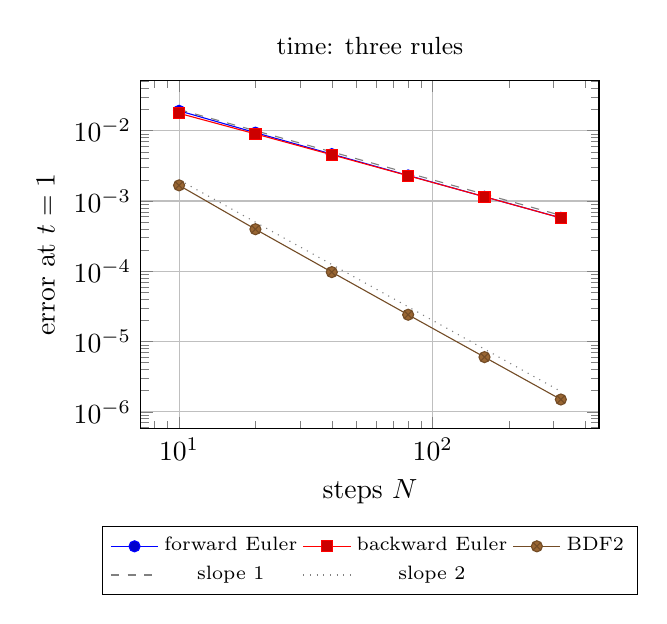
\begin{tikzpicture}
\begin{loglogaxis}[width=7.4cm, height=6cm, xlabel={steps $N$}, ylabel={error at $t=1$}, legend style={font=\scriptsize, at={(0.5,-0.28)}, anchor=north, legend columns=3}, grid=major, title={\small time: three rules}]
\addplot coordinates {(10,1.92e-2)(20,9.39e-3)(40,4.65e-3)(80,2.31e-3)(160,1.15e-3)(320,5.76e-4)}; \addlegendentry{forward Euler}
\addplot coordinates {(10,1.77e-2)(20,9.01e-3)(40,4.55e-3)(80,2.29e-3)(160,1.15e-3)(320,5.74e-4)}; \addlegendentry{backward Euler}
\addplot coordinates {(10,1.67e-3)(20,3.97e-4)(40,9.74e-5)(80,2.41e-5)(160,6.01e-6)(320,1.50e-6)}; \addlegendentry{BDF2}
\addplot[gray, dashed, domain=10:320] {0.2/x}; \addlegendentry{slope 1}
\addplot[gray, dotted, domain=10:320] {0.2/x^2}; \addlegendentry{slope 2}
\end{loglogaxis}
\end{tikzpicture}
\hfill
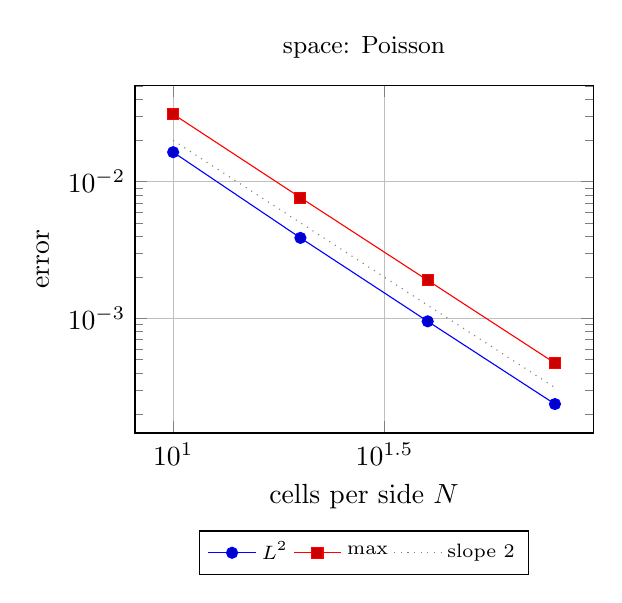
\begin{tikzpicture}
\begin{loglogaxis}[width=7.4cm, height=6cm, xlabel={cells per side $N$}, ylabel={error}, legend style={font=\scriptsize, at={(0.5,-0.28)}, anchor=north, legend columns=3}, grid=major, title={\small space: Poisson}]
\addplot coordinates {(10,1.64e-2)(20,3.88e-3)(40,9.53e-4)(80,2.37e-4)}; \addlegendentry{$L^2$}
\addplot coordinates {(10,3.11e-2)(20,7.64e-3)(40,1.90e-3)(80,4.72e-4)}; \addlegendentry{max}
\addplot[gray, dotted, domain=10:80] {2/x^2}; \addlegendentry{slope 2}
\end{loglogaxis}
\end{tikzpicture}
\caption{Convergence in time (left) and space (right).}
\label{fig:conv}
\end{figure}

\subsection{Cost and scaling}\label{sec:cost}

The timings in Table~\ref{tab:poisson} are the engineering result of this report. Quadrupling the cell count multiplies the three stages by (mesh derivation) $5.0$, $9.6$, $13.8$; (operator assembly) $14.9$, $16.5$, $19.2$; (GMRES solve) $5.0$, $8.4$, $10.7$. Expressed as exponents of the cell count $n$ on the last refinement, assembly scales as $n^{2.1}$, mesh derivation as $n^{1.9}$ and the unpreconditioned solve as $n^{1.7}$ (Figure~\ref{fig:cost}). Assembly dominates by two orders of magnitude at $6400$ cells, and its exponent is the quadratic cost of growing arrays by concatenation inside the fitted balance; a prior in-project profile attributed 97\% of one fit's 36\,$\mu$s to the stencil and CG machinery set up for a $4\times4$ system. The mesh derivation's exponent points to the face intersection. None of these is a property of the mathematics; each is a representation cost to be removed (Section~\ref{sec:future}).

\begin{figure}[H]
\centering
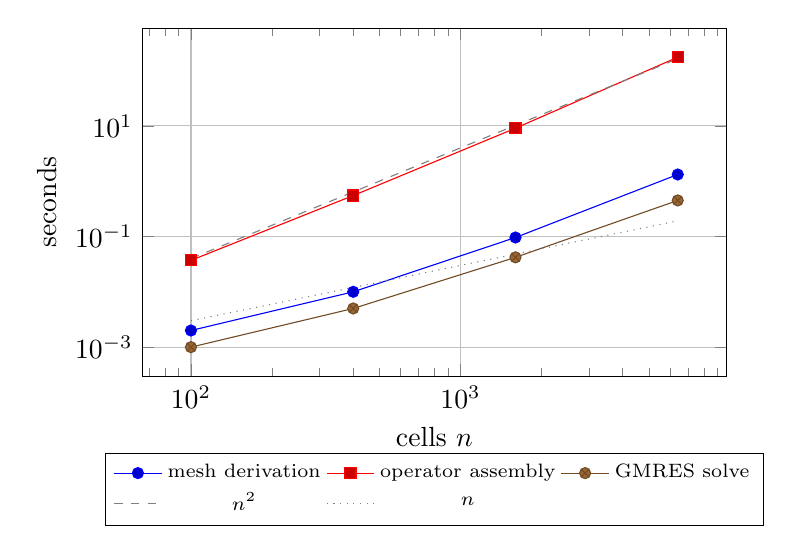
\begin{tikzpicture}
\begin{loglogaxis}[width=9cm, height=6cm, xlabel={cells $n$}, ylabel={seconds}, legend style={font=\scriptsize, at={(0.5,-0.22)}, anchor=north, legend columns=3}, grid=major]
\addplot coordinates {(100,0.002)(400,0.010)(1600,0.096)(6400,1.321)}; \addlegendentry{mesh derivation}
\addplot coordinates {(100,0.037)(400,0.550)(1600,9.077)(6400,174.285)}; \addlegendentry{operator assembly}
\addplot coordinates {(100,0.001)(400,0.005)(1600,0.042)(6400,0.449)}; \addlegendentry{GMRES solve}
\addplot[gray, dashed, domain=100:6400] {4e-6*x^2}; \addlegendentry{$n^2$}
\addplot[gray, dotted, domain=100:6400] {3e-5*x}; \addlegendentry{$n$}
\end{loglogaxis}
\end{tikzpicture}
\caption{Wall-clock cost per stage against cell count. Assembly is quadratic; the target for every stage is linear in cells plus faces.}
\label{fig:cost}
\end{figure}

\subsection{The source as an artefact}

Table~\ref{tab:metrics} records the source's shape. Three numbers characterize the design discipline: 68\% of procedures are \code{pure}; 191 \code{error stop}s each state the law whose violation they refuse; and the dependency graph of the 63 modules has 245 edges (12\% of the possible), a median module imported by one other, and a foundation of six modules (token, kernel graph, the set maps) whose transitive reach is 39--53 modules.

\begin{table}[H]
\centering\footnotesize
\begin{tabular}{@{}p{4.6cm}r@{\qquad}p{4.6cm}r@{}}
\toprule
modules & 63 & procedures & 375 \\
source lines & 21\,450 & \code{pure} procedures & 256 (68\%) \\
comment lines & 5\,858 (27\%) & \code{error stop} invariants & 191 \\
abstract types & 15 & deferred procedures & 79 \\
\code{extends} sites & 39 & dependency edges (density) & 245 (12\%) \\
modules: graph, token, relation, field & 1, 1, 5, 4 & modules: operation, transform, map, view, util & 26, 5, 7, 11, 3 \\
commits & 605 & history & 2018-11-15 to 2026-08-21 \\
compiler & \multicolumn{3}{l}{gfortran 15.2, \code{-std=f2023}} \\
\bottomrule
\end{tabular}
\caption{Source metrics on 22 August 2026.}
\label{tab:metrics}
\end{table}

\subsection{The two unification slices}

The measurements above were made after two changes completed on 21--22 August 2026 that made the composition and adjoint laws domain-generic: the stencil became the one affine sparse map (rectangular, with composition and transpose written once; the differential operator's private copy and the linearization's basis-built dual were deleted), and the marcher's per-instant tangent and adjoint solves became \code{implicit\_forward} and \code{implicit\_dual}. The suites were held at 159/159 across both; the source grew by 136 lines net, because rectangular maps with domains and the two generic solves cost more than the deleted second roads returned.

\section{Discussion: what is novel, and what is different}\label{sec:discussion}

\paragraph{Structure as the differentiation mechanism.} The established routes to discrete adjoints differentiate programs (source transformation, overloading, compiler passes) or record them (tapes). \ufvm{} differentiates \emph{statements}: an operation declares its exact partial actions, and the adjoint of a compiled operator is the transpose of a composition that already exists. There is no second program to verify; the adjoint's correctness is Proposition~\ref{prop:norev} plus the correctness of one transpose. The price is that a statement's author must write its partials; the reward is that every derived object---Jacobian, adjoint, directional derivatives of any order---costs nothing further.

\paragraph{Higher-order derivatives by partitions.} Taped systems obtain second derivatives by taping the tangent, and higher orders become unwieldy. The chain rule over integer partitions assembles any order directly from partial actions and is the same code for degree 1 and degree 8 (the suite checks degree 8 against a Taylor-convolution oracle in exact rationals).

\paragraph{Time and space as one.} The implicit function theorem at a vertex is the local law of both a time step and a steady residual; the marcher is a traversal that calls it. This is the structural reading of the graph-time-integration idea---compose once, dualize instead of reimplementing, solve locally---and Sections~\ref{sec:ift}--\ref{sec:marcher} are its realization in code rather than a claim.

\paragraph{The derived mesh and the relational matrix.} Deriving incidence from one relation is known; carrying identity on relations and sets, so that a partition is one relation read two ways and a wrong relation is refused by identity rather than by size, is the unusual part. Likewise a matrix as a weighted relation with a derived pattern is what makes the Galerkin coarse operator a relabelling and the adjoint a swap of two index arrays.

\paragraph{Parallel correctness before parallelism.} The four-step reduction, the image-aware token, the owned/borrowed partition and the exact round-trip law are all designed for a graph in pieces; none of the source is parallel today. This is a deliberate ordering: the laws that make a distributed run correct are in place before the runtime exists.

\paragraph{What is different, honestly.} The frameworks of Section~\ref{sec:related} offer vastly more physics, scale and tooling. \ufvm{} offers a smaller thing: a demonstration, with measurements, that a finite-volume solver with exact sensitivities of any order can be generated from eight types and a handful of laws, in 21\,000 lines of a language with no runtime dependencies beyond a Fortran compiler.

\section{Engineering assessment}\label{sec:assessment}

\paragraph{Strengths.}
\begin{itemize}[nosep]
\item Invariants are in the type system: private components and constructor-only introduction make the kernel's iff and token unforgeability unbreakable from outside; 191 stated refusals catch the rest at run time.
\item Derivatives are verified to machine precision against closed forms, not against themselves.
\item The build order is a dependency proof, checked mechanically along with the naming law on every commit.
\item Every module states its laws, its costs parametrically, and what it does \emph{not} do.
\end{itemize}

\paragraph{Limitations found in this assessment.}
\begin{itemize}[nosep]
\item Operator assembly is quadratic in cells (Table~\ref{tab:poisson}); at $6400$ cells it is $400\times$ the solve.
\item The Krylov solvers are unpreconditioned; multigrid is two-grid and attaches only to a compiled stencil.
\item The marcher solves every implicit block with dense direct elimination by basis evaluation---$n$ applications of the tangent per step---which is correct and exact for small states and unusable for large ones; the generic solves accept any minimizer, so the marcher needs only to pass one.
\item The in-repository test tree and documentation were deleted on 21 August 2026; the 159 checks reported here run from a copy restored by \code{maths/oracle.sh}, not from the tree, and the pre-commit hook references a coding standard that no longer exists in the tree.
\item The distributed runtime is designed but absent: no coarray statement exists in the source; the parallel build script references a deleted module.
\item The mesh loader reads MSH~4.1 only; geometric refinement has no positions and asserts only what connectivity supports.
\item gfortran enforces F2018~C1594, so procedures that copy a domain graph are impure; one banner claimed otherwise and was corrected.
\end{itemize}

\section{Conclusions}\label{sec:conclusions}

\ufvm{} demonstrates that a finite-volume simulation library can be generated from a small set of prime mathematical objects and that doing so turns laws into deletions: no reversed kernels, no hand Jacobians, no second CSR, no sparse-matrix class, no stored dependency pattern, no integrator-specific adjoint, no order-specific derivative code. The derived mesh, the weighted-relation matrix, the parity chain, the chain rule over partitions and the implicit function theorem at a vertex are each realized once and verified: nominal orders of accuracy in time and space, adjoints and higher-order directional derivatives exact to machine precision, and 159 structural properties holding on the current tree. The assessment is equally clear about cost: assembly is quadratic, solves are unpreconditioned, and the test tree must return to the repository. None of these touches the mathematics; all of them are representation work with a known target.

\section{Future work, from an engineering perspective}\label{sec:future}

\begin{enumerate}[nosep]
\item \textbf{Linear-cost assembly.} Replace array concatenation in the fitted balance with counted allocation, and solve the per-edge $4\times4$ fit by a dense local kernel rather than through the stencil/CG machinery. Target: assembly linear in faces; expected gain $\ge 100\times$ at $6400$ cells.
\item \textbf{Linear-cost mesh derivation.} Replace the pairwise face intersection with a hash of sorted vertex tuples; target $n^{1.0}$.
\item \textbf{Preconditioning and algebraic multigrid.} Jacobi/Gauss--Seidel preconditioners for CG/GMRES from the existing diagonal probe and colouring; multilevel aggregation from the two-grid Galerkin road.
\item \textbf{Sparse block solves in the marcher.} Pass a Krylov minimizer to \code{implicit\_forward} and \code{implicit\_dual} and drop the dense basis compile for large states; compile the block once per edge and reuse it across orders and the adjoint.
\item \textbf{The traversal on a DAG.} Generalize the marcher from a chain to any dependency graph in topological order, with the local statement taking one argument per in-edge; this makes space-marching and branching trajectories instances of the same traversal.
\item \textbf{More schemes by composition.} DIRK stages and Adams correctors as scaled backward steps against an externally assembled base, which the scheme already admits; Crank--Nicolson is present through $\theta=\tfrac12$.
\item \textbf{The distributed runtime.} Coarray halo exchange over the partition relation, with the four-step reductions and image-aware tokens already in place; restore and measure the parallel build.
\item \textbf{Restore the test tree and documentation in-repository}, applying the three mechanical API changes of this period (derived pattern, array weights, compiled dual; Appendix~\ref{app:api}), and regenerate the architecture map from the source.
\item \textbf{Enforce the stated-only laws} ($P\tr{}\tr=P$ extensionally, $L^{**}=L$ on the linear part, the round trip) as suite properties rather than prose.
\item \textbf{Hot-path measurement discipline.} Keep the small-$n$ gate (the ratio of a generic path to its direct equivalent) as a test, so representation changes are admitted by measurement.
\end{enumerate}

\appendix
\section{Interface changes applied by the oracle script}\label{app:api}

The suites at \code{ddcf592} predate the unification of the affine map. \code{maths/oracle.sh} applies three mechanical changes before building them; a restored in-tree suite must apply the same.
\begin{center}\footnotesize
\begin{tabular}{@{}p{5.4cm}p{9.8cm}@{}}
\toprule
before & after \\
\midrule
\code{x \% pattern} & \code{call x \% dependencies(p)} --- the pattern is derived, not stored \\
\code{call x \% weights \% real\_vector(w)} & \code{w = x \% weights} (constants likewise) --- plain arrays \\
\code{call dual\_by\_basis(t, g, lambda, d)} & \code{stencil(t, g, width, column\_domain=c, column\_entries=n)}\newline then \code{\% transpose()}, or \code{implicit\_dual} \\
\bottomrule
\end{tabular}
\end{center}
A stencil that declares a column domain now refuses, by identity, an input field on any other set, however long; a test that builds a basis vector on a freshly derived pattern's vertex set must build it on \code{x \% column\_domain} instead.

\begin{thebibliography}{99}\footnotesize
\bibitem{weller1998} H. G. Weller, G. Tabor, H. Jasak, C. Fureby. A tensorial approach to computational continuum mechanics using object-oriented techniques. \emph{Computers in Physics} 12(6), 1998.
\bibitem{economon2016} T. D. Economon, F. Palacios, S. R. Copeland, T. W. Lukaczyk, J. J. Alonso. SU2: An open-source suite for multiphysics simulation and design. \emph{AIAA Journal} 54(3), 2016.
\bibitem{sagebaum2019} M. Sagebaum, T. Albring, N. R. Gauger. High-performance derivative computations using CoDiPack. \emph{ACM TOMS} 45(4), 2019.
\bibitem{logg2012} A. Logg, K.-A. Mardal, G. N. Wells (eds.). \emph{Automated Solution of Differential Equations by the Finite Element Method}. Springer, 2012.
\bibitem{rathgeber2016} F. Rathgeber et al. Firedrake: automating the finite element method by composing abstractions. \emph{ACM TOMS} 43(3), 2016.
\bibitem{anderson2021} R. Anderson et al. MFEM: A modular finite element methods library. \emph{Computers \& Mathematics with Applications} 81, 2021.
\bibitem{farrell2013} P. E. Farrell, D. A. Ham, S. W. Funke, M. E. Rognes. Automated derivation of the adjoint of high-level transient finite element programs. \emph{SIAM J. Sci. Comput.} 35(4), 2013.
\bibitem{mitusch2019} S. K. Mitusch, S. W. Funke, J. S. Dokken. dolfin-adjoint 2018.1: automated adjoints for FEniCS and Firedrake. \emph{J. Open Source Software} 4(38), 2019.
\bibitem{hindmarsh2005} A. C. Hindmarsh et al. SUNDIALS: Suite of nonlinear and differential/algebraic equation solvers. \emph{ACM TOMS} 31(3), 2005.
\bibitem{zhang2022} H. Zhang, E. M. Constantinescu, B. F. Smith. PETSc TSAdjoint: a discrete adjoint ODE solver for first-order and second-order sensitivity analysis. \emph{SIAM J. Sci. Comput.} 44(1), 2022.
\bibitem{hascoet2013} L. Hascoët, V. Pascual. The Tapenade automatic differentiation tool: principles, model, and specification. \emph{ACM TOMS} 39(3), 2013.
\bibitem{griewank1996} A. Griewank, D. Juedes, J. Utke. ADOL-C: a package for the automatic differentiation of algorithms written in C/C++. \emph{ACM TOMS} 22(2), 1996.
\bibitem{moses2020} W. S. Moses, V. Churavy. Instead of rewriting foreign code for machine learning, automatically synthesize fast gradients. \emph{NeurIPS}, 2020.
\bibitem{jax2018} J. Bradbury et al. JAX: composable transformations of Python+NumPy programs, 2018.
\bibitem{griewank2008} A. Griewank, A. Walther. \emph{Evaluating Derivatives: Principles and Techniques of Algorithmic Differentiation}, 2nd ed. SIAM, 2008.
\bibitem{desbrun2005} M. Desbrun, A. N. Hirani, M. Leok, J. E. Marsden. Discrete exterior calculus. arXiv:math/0508341, 2005.
\bibitem{hirani2003} A. N. Hirani. \emph{Discrete Exterior Calculus}. PhD thesis, Caltech, 2003.
\bibitem{bell2012} N. Bell, A. N. Hirani. PyDEC: software and algorithms for discretization of exterior calculus. \emph{ACM TOMS} 39(1), 2012.
\bibitem{garimella2002} R. V. Garimella. Mesh data structure selection for mesh generation and FEA applications. \emph{Int. J. Numer. Meth. Engng} 55, 2002.
\end{thebibliography}

\end{document}
